\subsection{Programmablauf} % Johannes

\subsection{Partitionierung des Codes} % Flo
\begin{frame}
	\frametitle{Partitionierung des Codes}
	\framesubtitle{Grundlagen}
	\textbf{Ziel:} Finden von sinnvollen Übersetzungseinheiten
	
	\vspace{0.50cm}
	
	\textbf{Überlegung:}
	\begin{itemize}
		\item einzelne Instruktionen übersetzen zu aufwändig
		\item keine Übersetzung des ganzen Programmes
		\item[\conclude] Übersetzung von \textit{Basic Blocks}
	\end{itemize}
	
	\vspace{0.50cm}
	
	\begin{block}{Definition: Basic Block}
		\begin{itemize}
			\item einziger Ein- und Ausgangspunkt
			\item enthaltene Instruktionen der Reihe nach ausgeführt
		\end{itemize}
	\end{block}
\end{frame}

\begin{frame}
	\frametitle{Partitionierung des Codes}
	\framesubtitle{Finden von Blockgrenzen}
	
	\textbf{Blockende} durch folgende Instruktionen erreicht:
	\begin{itemize}
		\item Unbedingte Sprünge \& Funktionsaufrufe (\texttt{j}, \texttt{call}, \texttt{ret}) % todo I'll list the pseudos here, if that's fine?
		\item Bedingte Sprünge (\texttt{beq}, \texttt{bne}, \texttt{blt}, \texttt{bge}, \texttt{bltu}, \texttt{bgeu})
		\item System Calls (\texttt{ecall})
	\end{itemize}
	
	\vspace{0.50cm}
	
	\textbf{Optimierungspotenzial:}
	\begin{itemize}
		\item Sprüngen folgen
		\item rekursive Übersetzung von Sprungzielen
		\item Schwierigkeiten bei bedingten Sprüngen
	\end{itemize}
	
\end{frame}

\begin{frame}
	\frametitle{Partitionierung des Codes}
	\framesubtitle{Beispiel}

	\textbf{\color{blue} Sprungverfolgung} zu \texttt{\color{blue} label},\\
	\textbf{\color{red} Blockende} durch \texttt{\color{red}ecall}.

	\vspace{1.5cm}
	
	\begin{columns}[onlytextwidth]
		\ttfamily
		\begin{column}{0.49\textwidth}
			add  x6, x6, x7\\
			slli x6, x6, 3\\
			xori x7, x7, -1\\
			{\color{blue} j label}
		\end{column}
		
		\begin{column}{0.49\textwidth}
			{\color{blue} label:}\\
			addi a0, x0, 0\\
			addi a7, x0, \_\_NR\_exit\\
			{\color{red} ecall}
		\end{column}
	\end{columns}
\end{frame}


\subsection{Codegenerierung und Cache} % Flo
\begin{frame}
	\frametitle{Codegenerierung}
	\framesubtitle{Grundlagen}
	\textbf{Ziel:} Generieren von äquivalentem Code
	
	\vspace{0.50cm}
	
	\textbf{Prinzipieller Ansatz:} Instruktions-Mapping x86--64 \conclude RISC--V
	
	\begin{itemize}
		\item Übersetzungen jeder Instruktion der Quellarchitektur
		\item Probleme durch architektonische Unterschiede
		\begin{itemize}
			\item \textit{load-store}- vs. \textit{register-memory-Architektur}
			\item \textit{Zwei}- bzw. \textit{Dreiadressform}
		\end{itemize}
		
		\item Mustererkennung im Eingangscode
	\end{itemize}
\end{frame}

\begin{frame}
	\frametitle{Codegenerierung}
	\framesubtitle{Beispiel: Architektonische Unterschiede}
	
	\textbf{Problem:} ein Operand ist implizites Zielregister (x86)
	
	\vspace{2cm}
	
	\begin{columns}[onlytextwidth]
		\ttfamily
		\begin{column}{0.45\textwidth}
			\centering
			sub rd, rs1, rs2
		\end{column}
		
		\begin{column}{0.05\textwidth}
			\centering
			\conclude
		\end{column}
		
		\begin{column}{0.45\textwidth}
			\centering
			mov rd, rs1\\
			sub rd, rs2
		\end{column}
	\end{columns}
\end{frame}


\begin{frame}
	\frametitle{Codegenerierung}
	\framesubtitle{Beispiel: Optimierte Übersetzung}
	
	\textbf{Optimierungsmöglichkeit:} äquivalente native Instruktion existiert
	
	\vspace{2cm}
	
	\begin{columns}[onlytextwidth]
		\ttfamily
		\begin{column}{0.45\textwidth}
			\centering
			xori rd, rd, -1
		\end{column}
		
		\begin{column}{0.05\textwidth}
			\centering
			\conclude
		\end{column}
		
		\begin{column}{0.45\textwidth}
			\centering
			not rd
		\end{column}
	\end{columns}
\end{frame}


\begin{frame}
	\frametitle{Codegenerierung}
	\framesubtitle{Beispiel: Macro Operation Fusion}
	
	\textbf{Optimierungsmöglichkeit:} mehrere Instruktionen bündeln
	
	\vspace{2cm}
	
	\begin{columns}[onlytextwidth]
		\ttfamily
		\begin{column}{0.45\textwidth}
			\centering
			lui rd, imm1\\
			addi rd, rd, imm2
		\end{column}
		
		\begin{column}{0.05\textwidth}
			\centering
			\conclude
		\end{column}
		
		\begin{column}{0.45\textwidth}
			\centering
			mov rd, (imm1 + imm2)
		\end{column}
	\end{columns}
\end{frame}


\begin{frame}
	\frametitle{Code Cache}
	\framesubtitle{Konzept}
	
	\textbf{Hintergrund:} Angetroffene Basic Blocks sollen nur ein Mal übersetzt werden.
	
	\vspace{0.50cm}
	
	\begin{block}{Code Cache}
		\begin{itemize}
			\item Speicherregion, in die generierter Code geschrieben wird
			\item Index für die Speicherregion für schnellen Lookup (\refer Hash-Tabelle, TLB)
		\end{itemize}
	\end{block}
	
	\vspace{0.50cm}
	
	\textbf{Nutzung:}
	
	\begin{itemize}
		\item Block wird nach erstem Übersetzen in den Cache geschrieben
		\item Lookup vollzieht Adressübersetzung RISC--V \refer x86
		\item kein Löschen von übersetzten Blöcken (\refer Optimierungen)
	\end{itemize}
\end{frame}


\begin{frame}[c]
	\frametitle{Code Cache}
	\framesubtitle{Programmfluss (vereinfacht)}
	\centering
	\begin{figure}
		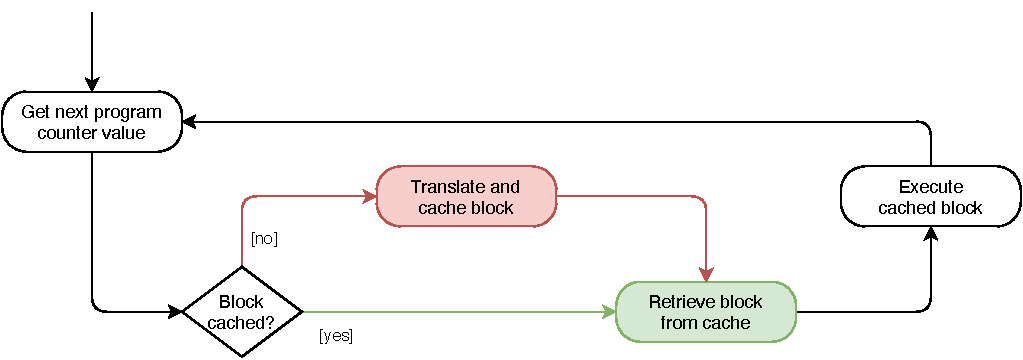
\includegraphics[width=\textwidth]{diagrams/cache-flow}
	\end{figure}
\end{frame}


\subsection{Registernutzung} % Flo
\begin{frame}
	\frametitle{Registernutzung}
	\framesubtitle{Grundlagen}
	
	\textbf{Ziel:} möglichst effizientes Emulieren der RISC--V-Register
	
	\vspace{0.50cm}
	
	\begin{block}{Definition: Registerdatei im Speicher}
		\begin{itemize}
			\item Speicherbereich, der die Registerwerte des Gastprogramms hält (264 Byte)
			\item Permanenter Speicherbereich, der über Kontextwechsel erhalten bleibt
		\end{itemize}
	\end{block}
	
	\vspace{0.50cm}
	
	\textbf{Problem:} viele Speicherzugriffe \conclude \alert{ineffizient}
\end{frame}

\begin{frame}
	\frametitle{Registernutzung}
	\framesubtitle{Ansatz}
	
	\textbf{Idee:} Werte in Registern halten
	
	\vspace{0.50cm}
	
	\begin{alertblock}{Register bei RISC--V und x86--64}
		\begin{columns}[onlytextwidth]
			\begin{column}{0.45\textwidth}
				\begin{itemize}
					\item \textbf{RISC--V}
					\begin{itemize}				
						\item 32 general-purpose Register
						\item \texttt{x0}, \texttt{x1}--\texttt{x31}
						\item festes Nullregister
					\end{itemize}
				\end{itemize}
			\end{column}
			
			\begin{column}{0.45\textwidth}
				\begin{itemize}
					\item \textbf{x86--64}
					\begin{itemize}				
						\item 16 general-purpose Register
						\item \texttt{rax}--\texttt{rdx}, \texttt{rsp}, \texttt{rbp}, \texttt{rsi}, \texttt{rdi}, und \texttt{r8}--\texttt{r15}
					\end{itemize}
				\end{itemize}
			\end{column}
		\end{columns}
	\end{alertblock}
	
	\vspace{0.50cm}
	
	\begin{itemize}
		\item zu wenige Register \conclude statische Abbildung nur teilweise möglich
		\item \texttt{rax}, \texttt{rcx}, \texttt{rdx} speziell benötigt; \texttt{rsp} unpraktisch
	\end{itemize}
\end{frame}

\begin{frame}
	\frametitle{Registernutzung}
	\framesubtitle{Ansatz}
	
	\textbf{Überlegung:} Welche 12 Register werden häufig verwendet?
	
\pgfplotstableread[col sep=comma,header=false]{../paper/benchmarks/register-frequency/freq.csv}\regfreqtable
\pgfplotstablesort[sort key =1, sort cmp=float >]\sortedregfreqtable{\regfreqtable}
\begin{figure}
%\pgfplotstabletypeset\sortedregfreqtable
	\centering
	\makebox[\textwidth][c]{
	\begin{tikzpicture}
		\begin{axis}[%
			ybar,
			area legend,
			ylabel = {Access percentage},
			xtick = data,
			xticklabel style = {
				inner sep = 0pt,
				anchor = north east,
				rotate = 60,
				font=\footnotesize
			},
			ytick = {0.1, 0.2, 0.3, 0.4},
			scaled y ticks = false,
			x = 0.4cm,
			point meta = {y*100},
			yticklabel = {\pgfmathparse{\tick*100}\pgfmathprintnumber{\pgfmathresult}\%},
			enlarge x limits = {abs = 0.5cm},
			xtick={0,...,31},
			xticklabels from table = {\sortedregfreqtable}{0},
			ymin = 0, ymax = 0.45,
			ymajorgrids = true,
			bar width = 5pt,
			bar shift = 0,
			height = 5.5cm,
			width = 0.85\linewidth,
			legend style = {
				at = {(0.98, 0.97)},
				anchor = north east,
				legend columns = 3,
				column sep = 0.2cm
			}
		]
			\addplot+[fill=era-dbt-1, draw=black, restrict x to domain=0:3]table [x expr = \coordindex, y = 1]\sortedregfreqtable;
			\addplot+[fill=era-dbt-2, draw=black, restrict x to domain=4:4]table [x expr = \coordindex, y = 1]\sortedregfreqtable;
			\addplot+[fill=era-dbt-1, draw=black, restrict x to domain=5:12]table [x expr = \coordindex, y = 1]\sortedregfreqtable;
			\addplot+[fill=era-dbt-2, draw=black, restrict x to domain=13:31]table [x expr = \coordindex, y = 1]\sortedregfreqtable;

			\legend{statically mapped, not mapped}
		\end{axis}
	\end{tikzpicture}
	}
\end{figure}
\end{frame}

\begin{frame}
	\frametitle{Registernutzung}
	\framesubtitle{Vorgehen}
	
	\textbf{Idee:} Speicherzugriffe minimieren
	
	\vspace{0.50cm}
	
	\begin{block}{Register-Handling-Strategie}
		\begin{itemize}
			\item statische Abbildung der 12 zugriffshäufigsten Register (außer \texttt{x0})
			\begin{itemize}
				\item \texttt{a0}--\texttt{a5}, \texttt{a7}, \texttt{s1}--\texttt{s2}, \texttt{ra}, \texttt{fp}, \texttt{sp}
				\item bleiben über Blockgrenzen hinweg erhalten (\refer Kontextwechsel)
			\end{itemize}
			
			\item dynamische Allokation in die restlichen 3 x86-Register
			\begin{itemize}
				\item dynamisch in \texttt{rax}, \texttt{rcx}, \texttt{rdx} (\textit{least recently used}, \textit{lazy write-back})
				\item an Blockgrenzen zurückgeschrieben
			\end{itemize}
		\end{itemize}
	\end{block}
	
\end{frame}


\subsection{Optimierungen} % Johannes

